Our experiments are based on Social Ways. A major change in Social Ways compared to previously implemented GAN models for trajectory prediction is that it implements the InfoGAN architecture. The results from Social Ways~\cite{DBLP:journals/corr/abs-1904-09507} show that InfoGAN can greatly improve the trajectory prediction of multimodal pedestrians, avoiding pattern collapse and degradation. Figure~\ref{socialways} illustrates the architecture.

\begin{figure*}[ht]
  \centering
  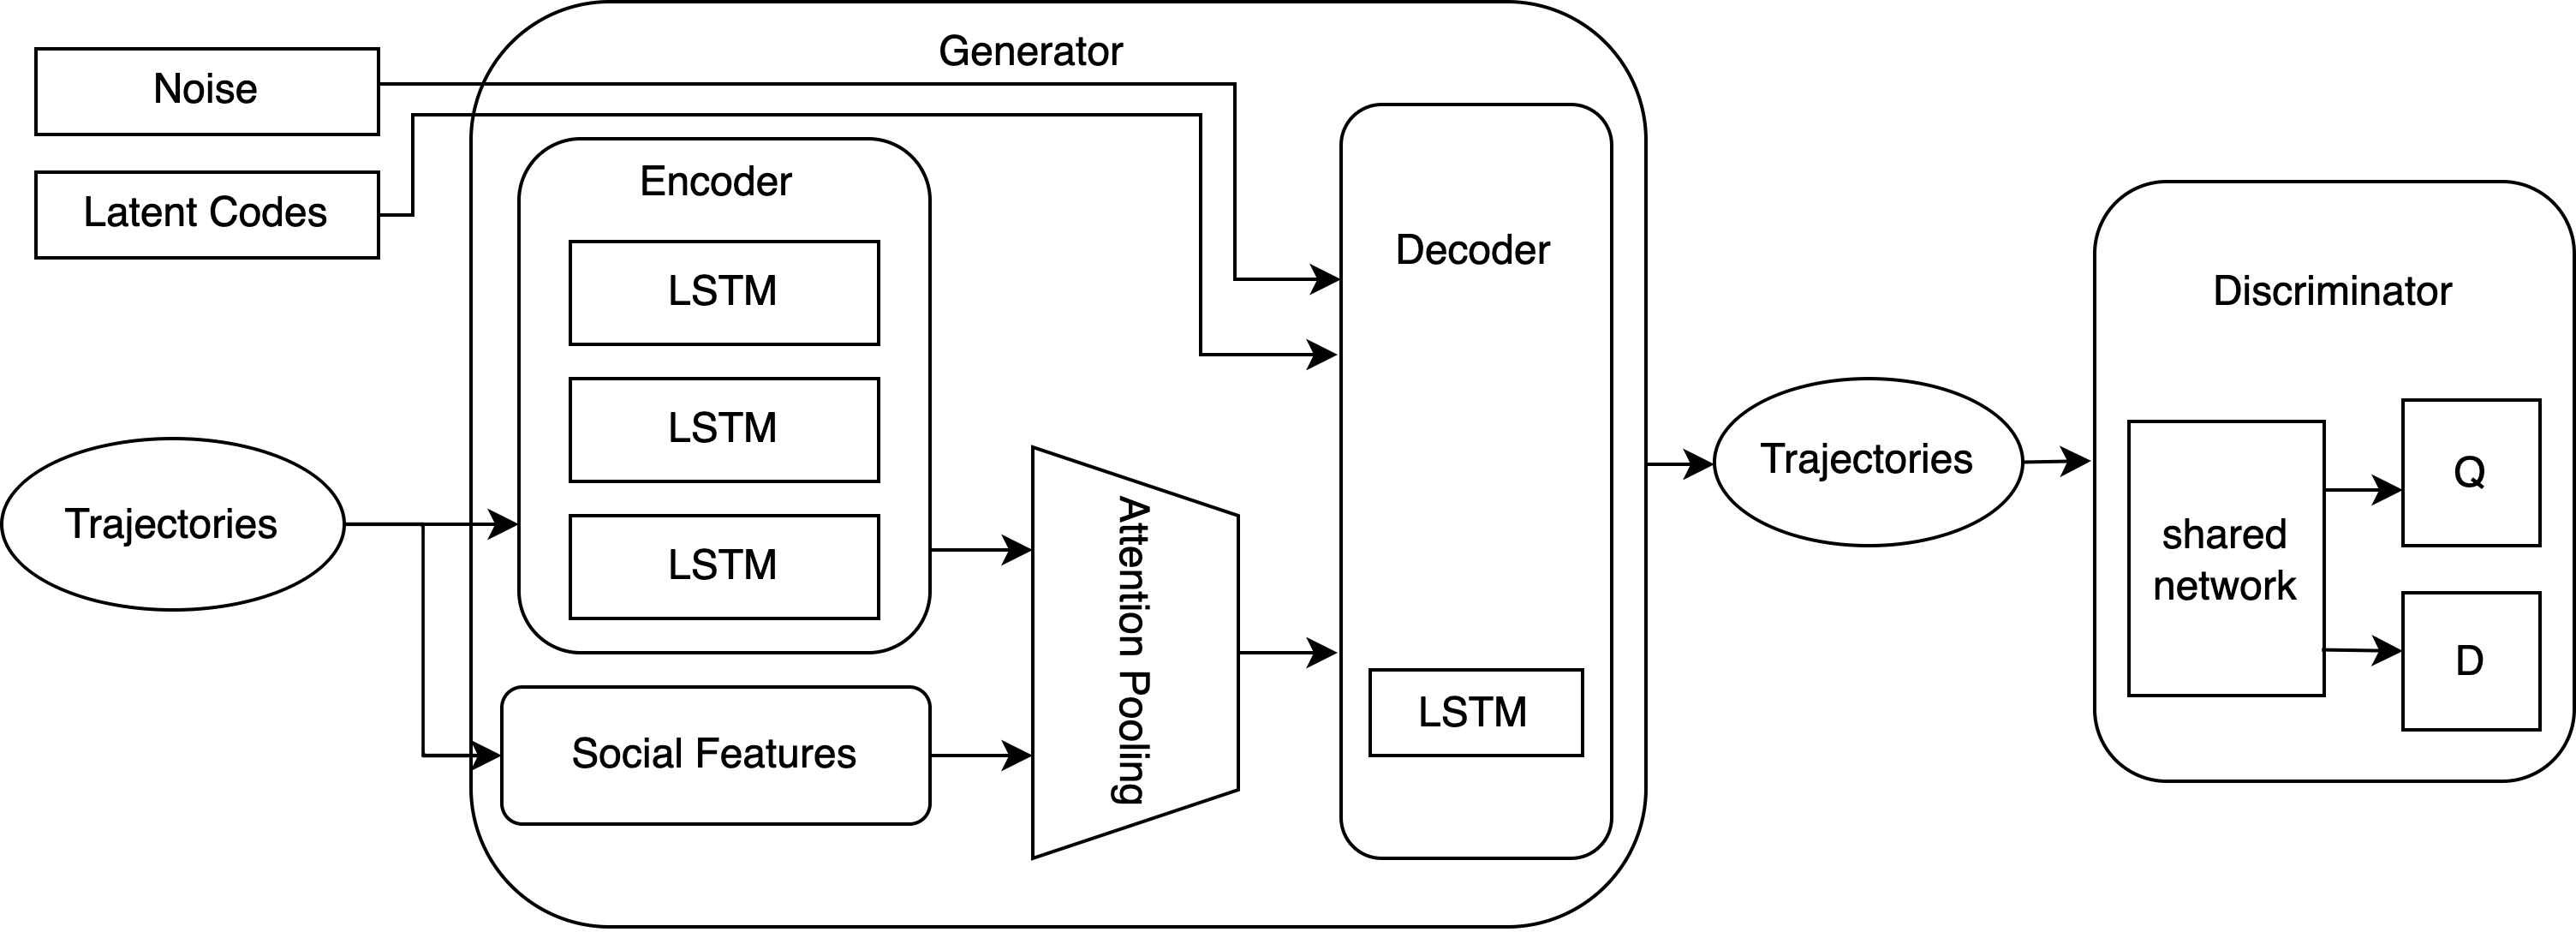
\includegraphics[width=0.8\textwidth]{figures/socialways.png}
  \caption{Architecture of Social ways}
  \Description{Figure from Social Ways}
  \label{socialways}
\end{figure*}

In the following subsections, we will describe the key methods of Social Ways and our experiments.

\subsection{Methodology}


\subsubsection{Generative Adversarial Networks}
\hfill \\
According to the research of Generative Adversarial Nets~\cite{gan}: a Generative Adversarial Network (GAN) consists of two network components, a discriminator $D$ and a generator $G$, which compete with each other. $G$ takes the input noise variable $z$ and generates the sample $G(z)$, $D$ takes the generated sample or training data as input $x$ and predicts the probability $D(x)$ that $x$ comes from the data and not generated by $G$. $D$ is trained to maximize the probability of assigning correct labels to training samples and generated samples, while $G$ is trained to minimize the correctness of $D$. In other words, $D$ and $G$ play a min-max game with the value function $V(G, D)$.

\begin{multline}
  \min_{G} \max_{D} V(G, D) = \mathbb{E}_{x \sim p_{\text{data}}} \lbrack \log(D(x))\rbrack \\ + \mathbb{E}_{z \sim p_{z}(z)} \lbrack \log(1 - D(G(z))) \rbrack
\end{multline}

In our case, for pedestrian trajectory data, the generator is trained to generate possible future trajectories that have a distribution similar to the training data, given certain previously observed trajectories, while the discriminator learns to distinguish the rationality of the generated paths. These two networks are trained simultaneously. As the discriminators are learned, the generators are improved.

\subsubsection{InfoGAN}


\subsubsection{Desciption of Latent Code}

\hfill \\
Our experiments attempt to disentangle the latent code so that the latent code can correspond to the semantic features of the data. To enrich our expression, we allow two types of latent codes, categorical latent codes and continuous latent codes.

For categorical latent code $c$, we can use cross entropy as a loss function to maximize the information between the code and the code predicted by $Q$.


$$\mathcal{L} (c, Q(G(x, c))) = MSE(c, Q(G(x, c))) $$

For a continuous latent code $c$, we can use the mean squared error as a loss function to maximize the information between the code and the code predicted by $Q$.

$$\mathcal{L} (c, Q(G(x, c))) = CE(c, Q(G(x, c))) $$

On the basis of categorical latent codes and continuous latent codes, we can introduce a series of semantic factors. For example, velocity and direction can be represented as continuous latent codes and scenes can be expressed as categorical latent codes. For map/obstacle information, the image embedding of the background image (the background image of the video recording trajectory data) can be used as a sequence of continuous latent codes.